\documentclass[11pt,a4paper,oneside,ngerman]{article}

\usepackage[left=2.5cm,right=2.5cm,top=2.5cm,bottom=2.5cm]{geometry}

\usepackage{lmodern}									% Latin Modern
\renewcommand*\familydefault{\sfdefault} 			% Only if the base font of the document is to be sans serif
\usepackage[T1]{fontenc}

\usepackage[ngerman]{babel}							% Setzt die deutsche Sprache, sodass statt table of contents
													% Inhaltsverzeichnis geschrieben wird
\usepackage[utf8]{inputenc}    						% Koderiung: UTF-8
\usepackage{color}									% Ermöglicht farbigen Text: \textcolor{declared-color}{text}
													% Bsp.: \textcolor{red}{Dieser Text ist rot}	
\usepackage{graphicx}					
\usepackage{wrapfig}									% Ermöglicht Bildumlauf mit der wrapfigure-Umgebung
\usepackage{mathtools}
\usepackage{listings}								% Erlaut das einfügen von Quell-Code
										
\usepackage{fancyhdr} 
%\pagestyle{fancy}
\fancyhf{} 											% alle Kopf- und Fußzeilenfelder bereinigen;
													% löscht doppelte Seitenzahlen!
%\fancyhead[L]{} 									% Kopfzeile links
%\fancyhead[C]{}										% zentrierte Kopfzeile
%\fancyhead[R]{} 									% Kopfzeile rechts
\fancyfoot[R]{\thepage}				 				% Seitennummer

%\renewcommand{\headrulewidth}{0.4pt} %obere Trennlinie
%\renewcommand{\footrulewidth}{0.4pt} %untere Trennlinie			

\newcommand{\qr}{\textquotedblleft}				% Definiert eine Abkürzung für dt. Anführungsstriche links
\newcommand{\ql}{\quotedblbase}					% Definiert eine Abkürzung für dt. Anführungsstriche rechts

%%% Generelle Inforationen über das Dokument

\author{Kilian Engelhardt}
\title{Zusammenfassung d. Berufsschulunterrichts}
\date{\today}

\usepackage{hyperref}						% Weitere Optionen unter:
											% http://de.wikibooks.org/wiki/LaTeX-W%C3%B6rterbuch:_hyperref
\hypersetup{									% Hier werden Informationen für das PDF gesetzt
pdftitle={},
pdfauthor={},
pdfsubject={},
pdfkeywords={},
colorlinks=true,							
linkcolor=black								% Definiert die Farbe der Links vom Inhaltsverzeichnis
}											% zu den Sections im Dokument

%%% Beginn des Inhalts

\begin{document}

	\begin{center}
		\Huge{Zusammenfassung: Jahr 1}
	\end{center}

%\pagestyle{empty}	
%\include{zusammenfassung-deckblatt}
\tableofcontents
\newpage
\pagestyle{fancy}
\setcounter{page}{1}

% Die Lernfelder werden hinzugefügt 
\section{Lernfeld 1A - Betrieb und sein Umfeld}

\subsection{Einführung}
Im Lernfeld 1A \ql Betrieb und sein Umfeld\qr\ werden sowohl Aspekte der Volkswirtschaftslehre (VWL) als auch Betriebswirtschaftslehre (BWL) besprochen. Dabei handelt es sich im Groben um die marko- und mirkoökonomischen Aspekte des wirtschaftlichen Handelns.

In der VWL werden Indikatoren behandelt, welche dazu dienen sollen, die gesamtwirtschaftliche Leistung eines Landes zu messen. Im Kontrast dazu behandelt die BWL Indikatoren zur Bestimmung der Leistung einzelner Unternehmen.

Privatwirtschaftliche Akteure können verschiedene Ziele haben, beispielsweise Gewinnmaximierung oder Gewinnung von Marktanteilen. Öffentliche Akteure stellen in erster Linie Infrastruktur bereit, wie zum Beispiel das Straßenverkehrsnetz.

Allgemein ist wirtschaftendes Handeln notwendig, da die Ressourcen auf unserer Erde begrenzt sind. Dabei gibt es zwei hervorstechende Prinzipien: erstens das {\bf Minimal-Prinzip} und zweitens das {\bf Maximal-Prinzip}. Dem Minimal-Prinzip folgend wird versucht ein festes Ziel mit möglichst wenig Ressourceneinsatz zu erreichen. Beim Maximal-Prinzip wird versucht mit einer festen Menge von Ressourcen ein möglichst großes Ziel zu erreichen.

Warum müssen wir überhaupt wirtschaften? Wir müssen wirtschaften, weil wir Bedürfnisse haben. Die Darstellung von Bedürfnissen erfolgt meist in der Form einer Pyramide. Die wohl bekannteste dieser Darstellung ist die Maslowsche Bedürfnishierarchie.

Produktionsfaktoren sind

%%% Marktstruktur und Auswirkungen
% Angebot und Nachfrage, Marktarten, Preisbildung, Preiseingriffe d. Staates:

Außerdem werden im Lernfeld die Themen Marktstruktur und ihre Auswirkungen auf das Handeln der Marktteilnehmer besprochen. Grob gesprochen gibt es zwei Arten von Märkten: zum einen den {\bf Käufermarkt} und zum anderen den {\bf Verkäufermarkt}. Auf dem Käufermarkt sind die Käufer im Vorteil, weil es beispielsweise mehr Angebot als Nachfrage gibt. Auf einem Verkäufermarkt sind die oder der Verkäufer im Vorteil, da diese oder dieser ein Monopol durch Patente auf ein gefragtes Produkt hält und so ein geringes Angebot mit hoher Nachfrage besteht.

Durch Angebot und Nachfrage wird der Preis eines Produktes bestimmt. Die folgende Grafik beschreibt die Entstehung des Gleichgewichtspreis.

%%% Anfang: Gleichgewichtspreis
\begin{wrapfigure}{l}{0.3\textwidth}
	\begin{center}
		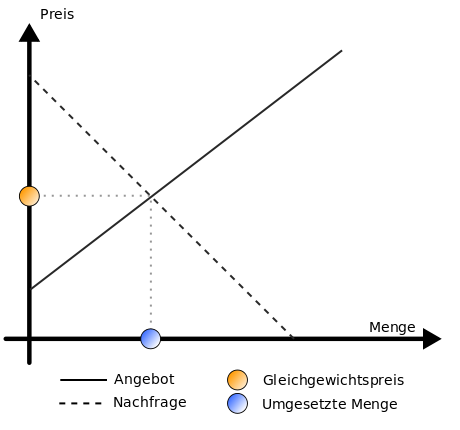
\includegraphics[width=0.28\textwidth]{pictures/lf01-pic/lf01-gleichgewichtspreis.png}
	\end{center}
	\caption{Entstehung des Gleichgewichtspreis}
\end{wrapfigure}
%%% Ende

Die Angebotslinie startet mit kleinem Angebot bei einem niedrigen Minimalpreis und wächst mit steigendem Preis. Die Nachfragelinie startet mit einer kleinen Nachfrage bei einem hohen Maximalpreis und nimmt mit fallendem Preis immer weiter an Menge zu. Wie an diesen zwei Linien zu erkennen ist, gibt es immer mehr Anbieter und Ware je höher der verlangte Preis ist. Umgekehrt gibt es immer mehr Abnehmer, die immer mehr kaufen, je niedriger der für die Ware verlangte Preis ist. Da die Preiswünsche von Anbietern und Abnehmern gegenläufig sind, stellt sich im Markt ein Gleichgewicht an der Schnittstelle von Angebot und Nachfrage ein, die den Gleichgewichtspreis und das Maximum des Umsatzes festlegt.

Marktsättigung führt dazu, dass kontinuierlich neue Produkte entwickelt werden müssen. Ein hilfreiches Instrument, um eine dauerhafte Marktsättigung zu umgehen, ist die geplante Obsoleszenz. Es werden absichtlich Bauteile verwendet, die nur eine begrenzte Lebenszeit haben; idealerweise beträgt die Lebenszeit eines solchen Bauteils nicht länger als die gesetzlich vorgeschriebene Garantiezeit. Dadurch wird eine konstante Nachfrage generiert.


%%% Kooperation und Konzentration: Monopol, Oligopol

%%% Grundzüge staatlicher Wirtschaftspolitik

%%% Anfang: Werbung
\subsection{Werbung}

Was versteht das Recht unter sogenannten \ql Lockangeboten\qr? Welche Art von Werbung ist erlaubt und welche nicht? Diese und weitere Fragen werden in diesem Abschnitt beantwortet.

Für beworbene Waren gilt eine Vorratsfrist von zwei Tagen. In Ausnahmen darf diese auch weniger getragen, beispielsweise wenn die Höhe der Nachfrage nicht absehbar war. Die Formulierung \ql Solange der Vorrat reicht\qr\ hebelt die Vorratsfrist aus, aber nur falls keine Vorerfahrung über die Höhe der Nachfrage bestand.

Das Gesetz gegen unlauteren Wettbewerb (UWG) regelt, welche Formen der Werbung erlaubt sind und unter welchen Umständen sie als unlauter gelten.

Der Zweck von Lockangeboten besteht darin, Kunden in den Laden zu locken. Diese kommen bereits mit einer Kaufabsicht in den Laden. Wenn dann das beworbene Angebot nicht mehr erhältlich ist, greifen viele dieser Kunden zu einem ähnlichen aber teureren Produkt. 

Vergleichende Werbung ist nur in wenigen Fällen unproblematisch, sodass meistens darauf verzichtet wird.

Unter \ql Mondpreiswerbung\qr\ wird eine künstliche Erhöhung des Preises verstanden, um anschließend mit einer Reduzierung des Preises zu werden. Preise müssen normalerweise 6 Monate lang konstant bleiben.

Außerdem fällt unzumutbare Belästigung in den Bereich des unlauteren Wettbewerbs.

Im Einzelnen wurden die Paragraphen 3 bis 7 des UWG besprochen. Die Überschriften der Paragraphen lauten:
\begin{itemize}
	\item[§3] Verbot unlauterer geschäftlicher Handlungen
			\begin{itemize}
				\item Interessen von Mitbewerbern, Verbrauchern oder sonstigen Marktteilnehmern dürfen nicht spürbar beeinträchtigt werden.
				\item Geschäftliche Handlungen gegenüber Verbrauchern sind unzulässig, wenn sie nicht der für den Unternehmer geltenden fachlichen Sorgfalt entsprechen.
				\item Die Fähigkeit des Verbrauchers, sich auf Grund von Informationen zu entscheiden, darf nicht spürbar beeinträchtigt werden. Er darf nicht zu einer geschäftlichen Entscheidung veranlasst werden, die er sonst nicht getroffen hätte.
			\end{itemize}
	\item[§4] Beispiele unlauterer geschäftlicher Handlungen
			\begin{enumerate}
				\item Entscheidungsfreiheit der Marktteilnehmer durch Ausübung von Druck, in menschenverachtender Weise oder durch sonstigen unangemessenen unsachlichen Einfluss zu beeinträchtigen.
				\item Ausnutzen von geistigen oder körperlichen Gebrechen, des Alters, der geschäftlichen Unerfahrenheit, der Leichtgläubigkeit, der Angst oder der Zwangslage des Marktteilnehmers
				\item Verschleierung des Werbecharakters geschäftlicher Handlungen
				\item Bedingungen für die Inanspruchname von Verkaufsförderungsmaßnahmen wie Preisnachlässen, Zugaben oder Geschenken werden nicht klar und eindeutig angegeben
				\item Teilnahmebedingungen werden bei Preisausschreiben oder Gewinnspielen mit Werbecharakter nicht klar und eindeutig angegeben
				\item Teilnahme von Verbrauchern an einem Preisausschreiben oder einem Gewinnspiel ist an den Erwerb einer Ware oder die Inanspruchname einer Dienstleistung abhängig. \\
{\it Ausnahme:} Das Preisausschreiben oder Gewinnspiel ist naturgemäß mit der Ware oder Dienstleistung verbunden
				\item Die Kennzeichen, Waren, Dienstleistungen, Tätigkeiten oder persönlichen geschäftlichen Verhältnisse eines Mitbewerbers werden herabgesetzt oder verunglimpft			
				\item über die Waren, Dienstleistungen oder das Unternehmen eines Mitbewerbers oder über Unternehmer oder ein Mitglied der Unternehmensleitung Tatsachen behaupten oder verbreiten, die geeignet sind, den Betrieb des Unternehmens oder den Kredit des Unternehmers zu schädigen, sofern die Tatsachen nicht erweislich wahr sind.
			\end{enumerate}
	\item[§5] Irreführende geschäftliche Handlungen
		\begin{itemize}
			\item Eine geschäftliche Handlung ist Irreführend, wenn sie unwahre Angaben enthält oder sonstige zur Täuschung geeigneten Angaben über die wesentlichen Merkmale der Ware oder Dienstleistung oder den Anlass des Verkaufs enthält
			\item Verwechslungsgefahr mit einer anderen Ware oder Dienstleistung oder mit der Marke oder einem anderen Kennzeichen eines Mitbewerbers wird hervorgerufen
			\item Werbung mit einer Herabsetzung eines Preises, sofern der Preis nur eine unangemessen kurze Zeit gefordert worden ist ({\it Mondpreiswerbung})
		\end{itemize}
	\item[§5a] Irreführung durch Unterlassung
		\begin{itemize}
			\item Beeinflussung der Entscheidungsfähigkeit der Marktteilnehmer durch verschweigen wesentlicher Informationen
		\end{itemize}
	\item[§6] Vergleichende Werbung
		\begin{itemize}
			\item Vergleich bezieht sich nicht auf Waren oder Dienstleistungen für den gleichen Bedarf oder dieselbe Zweckbestimmung
			\item Nicht objektive auf wesentliche, relevante, nachprüfbare und typische Eigenschaften oder den Preis bezogen ist
			\item Verwechslung mit Mitbewerbern oder von diesen angebotenen Produkten
			\item Ruf des von einem Mitbewerber verwendeten Kennzeichen wird in unlauterer Weise ausgenutzt oder beeinträchtigt
			\item Ware oder Dienstleistung als Imitation oder Nachahmung einer unter einem geschützten Kennzeichen vertriebenen Ware oder Dienstleistung darstellen
		\end{itemize}
	\item[§7] Unzumutbare Belästigung
		\begin{itemize}
			\item Werbung, obwohl erkennbar ist, dass der angesprochene Marktteilnehmer diese Werbung nicht wünscht
			\item Werbung mit einem Telefonanruf gegenüber einem Verbraucher ohne dessen vorherige ausdrückliche Einwilligung
			\item Werbung unter Verwendung einer automatischen Anrufmaschine, eines Faxgeräts oder elektronischer Post, ohne vorherige ausdrückliche Einwilligung des Adressaten
			\item Verschleierung der Identität des Absenders
		\end{itemize}
\end{itemize}

%%% Ende: Werbung

%%%%%%%%%%%%%%%%%%%%%%%%%%%%%%%%%%%%%%%%%%%%%%%%%%%%%%%%%%%%%%%%%%%%%%%%%%%%%%%%

%%% Anfang: Betriebliche Kennzahlen
\subsection{Betriebliche Kennzahlen}

Als Kennziffern werden Indikatoren zur Bestimmung des wirtschaftlichen Erfolges bezeichnet, welche in Form von Zahlen ermittelt werden können. Dazu gehören offensichtliche Werte wie der Gewinn eines Unternehmens als auch die Produktivität. Betriebliche Kennzahlen können unter anderem in Relation zum Vorjahr, der Auslastung oder der Konkurrenz betrachtet werden.\\

%%% Formeln zur Berechnung der Kennziffern:

% Produktivität
Die Produktivität ist eine {\bf Messgröße für die Ergiebigkeit der in der Produktion eingesetzten Produktionsfaktoren}. \\
$Produktivität = \frac{mengenmäßige Ausbringungsmenge}{mengenmäßigen Einsatz der Produktionsfaktoren} = \frac{Output}{Input}$\\
$Arbeitsproduktivität = \frac{mengenmäßige Ausbringungsmenge}{Arbeitsstunden}$\\
\\
% Wirtschaftlichkeit
Bei der Berechnung der Wirtschaftlichkeit handelt es sich um eine Erweiterung der Produktivität um den Faktor Geld. Zur Berechnung der Wirtschaftlichkeit werden die wertmäßigen Leistungen auf den Wert der eingesetzten Produktionsfaktoren bezogen.\\
$Wirtschaftlichkeit = \frac{Leistungen}{Kosten}$\\
\\
% Produktivitätsfaktor
% Rentabilität
Die Erzielung von Gewinnen ist das Ziel privatwirtschaftlicher Unternehmen. Zur Beurteilung des Erfolges muss der Gewinn in Bezug zum eingesetzten Kapital gesetzt werden.\\
$Eigenkapitalrentabilität = \frac{Gewinn \times 100}{Eigenkapital}$\\
\\
Die Gesamtkapitalrentabilität zeigt an, wie sich das gesamte in der Unternehmung eingesetzte Kapital verzinst. Zur Erzielung von Gewinn aus dem eingesetzten Fremdkapital muss die Eigenkapitalrentabilität über dem Fremdkapitalzins liegen.\\
$Gesamtkapitalrentabilität = \frac{(Gewinn + Fremdkapital) * 100}{Eigenkapitel + Fremdkapital}$\\
\\
% Bilanzanalyse
% Investitionsanalyse
% Quoten
Die Eigenkapitalquote setzt das Eigenkapital in Bezug zum Gesamtkapital des Unternehmens.\\
$Eigenkapitalquote = \frac{Eigenkapital * 100}{Gesamtkapital}$\\
\\
Die Fremdkapitalquote setzt das eingebrachte Fremdkapital in Bezug zum Gesamtkapital des Unternehmens.\\
$Fremdkapitalquote = \frac{Fremdkapital * 100}{Gesantkapital}$\\
\\
Der Verschuldungsgrad gibt den Anteil des Fremdkapitals am Eigenkapital an.\\
$Verschuldungsgrad = \frac{Fremdkapital * 100}{Eigenkapital}$\\
\\
% Intensitäten
Die Anlageintensität gibt den Anteil des Anlagevermögens (dem Unternehmen dauerhaft dienend) am Gesamtvermögen an.\\
$Anlageintensität = \frac{Anlagevermögen * 100}{Gesamtvermögen}$\\
\\
Die Arbeitsintensität gibt den Anteil des Umlaufvermögens (dem Unternehmen kurzzeitig dienend, z.B. auf Lager liegende Waren) am Gesamtvermögen an.\\
$Arbeitsintensität = \frac{Umlaufvermögen * 100}{Gesamtvermögen}$\\
\\
% Finanzierungsanalyse
% Liquiditätsanalyse
Der Anlagendeckungsgrad I gibt an, welcher Anteil des Anlagevermögens durch Eigenkapital gedeckt ist. Nach der {\it Goldenen Bilanzregel im engeren Sinne} sollte das Anlagevermögen durch Eigenkapital finanziert werden.\\
$Anlagedeckungsgrad I = \frac{Eigenkapital}{Anlagevermögen}$\\
\\
Der Anlagendeckungsgrad II gibt an, welcher Anteil des Anlagevermögens durch Eigenkapital und langfristiges Fremdkapital gedeckt ist. Nach der {\it Goldenen Bilanzregel im weiteren Sinne} soll die Finanzierung durch langfristig zur Verfügung stehendes erfolgen.\\
$Anlagedeckungsgrad II = \frac{Eigenkapital + langfristiges Fremdkapital}{Analgevermögen}$\\
\\
%Liquidität
Die Liquidität ist eine Existenzbedingung des Unternehmens, die auch kurzfristig immer gesichert sein muss, um eine Zahlungsfähigkeit zu gewährleisten und eine eventuelle Gefahr für den Fortbestand durch Zahlungsunfähigkeit zu verhindern.\\
Flüssige Mittel = Kasse, Postgiroguthaben, Guthaben bei Kreditinstituten, Schecks, diskontfähige Wechsel und börsengängige Wertpapiere\\
Kurzfristige Forderungen = Forderungen mit einer Restlaufzeit bis zu einem Jahr\\
Kurzfristige Verbindlichkeiten = Verbindlichkeiten mit einer Restlaufzeit bis zu einem Jahr\\

$Liquidität 1. Grades = \frac{Flüssige Mittel * 100}{Kurzfristige Verbindlichkeiten}$\\
$Liquidität 2. Grades = \frac{(Flüssige Mittel + kurzfr. Forderungen) * 100}{Kurzfristige Verbindlichkeiten}$\\
$Liquidität 3. Grades = \frac{Umlaufvermögen * 100}{Kurzfristige Verbindlichkeiten}$\\

%%% Ende: Betriebliche Kennzahlen
%%%%%%%%%%%%%%%%%%%%%%%%%%%%%%%%%%%%%%%%%%%%%%%%%%%%%%%%%%%%%%%%%%%%%%%%%%%%%%%%

%%% Anfang: Wirtschaftskreislauf
\subsection{Wirtschaftskreislauf}

Der Wirtschaftskreislauf beschreibt den Austausch von Gütern, Dienstleistungen und Geld. Dadurch werden die Zusammenhänge der einzelnen Akteure (Unternehmen, Haushalte, Banken, Staaten \dots) deutlich.

Manchmal werden Preise mit negativem Deckungsbeitrag -- das sind Preise, die unter den Produktionskosten liegen -- ausgeschrieben, um beispielsweise eine stärkere Marktdurchdringung oder eine Verdrängung von Konkurrenz zu erreichen. Ein negativer Deckungsbeitrag wird auch verwendet, um seine Lagerbestände zu leeren. \\
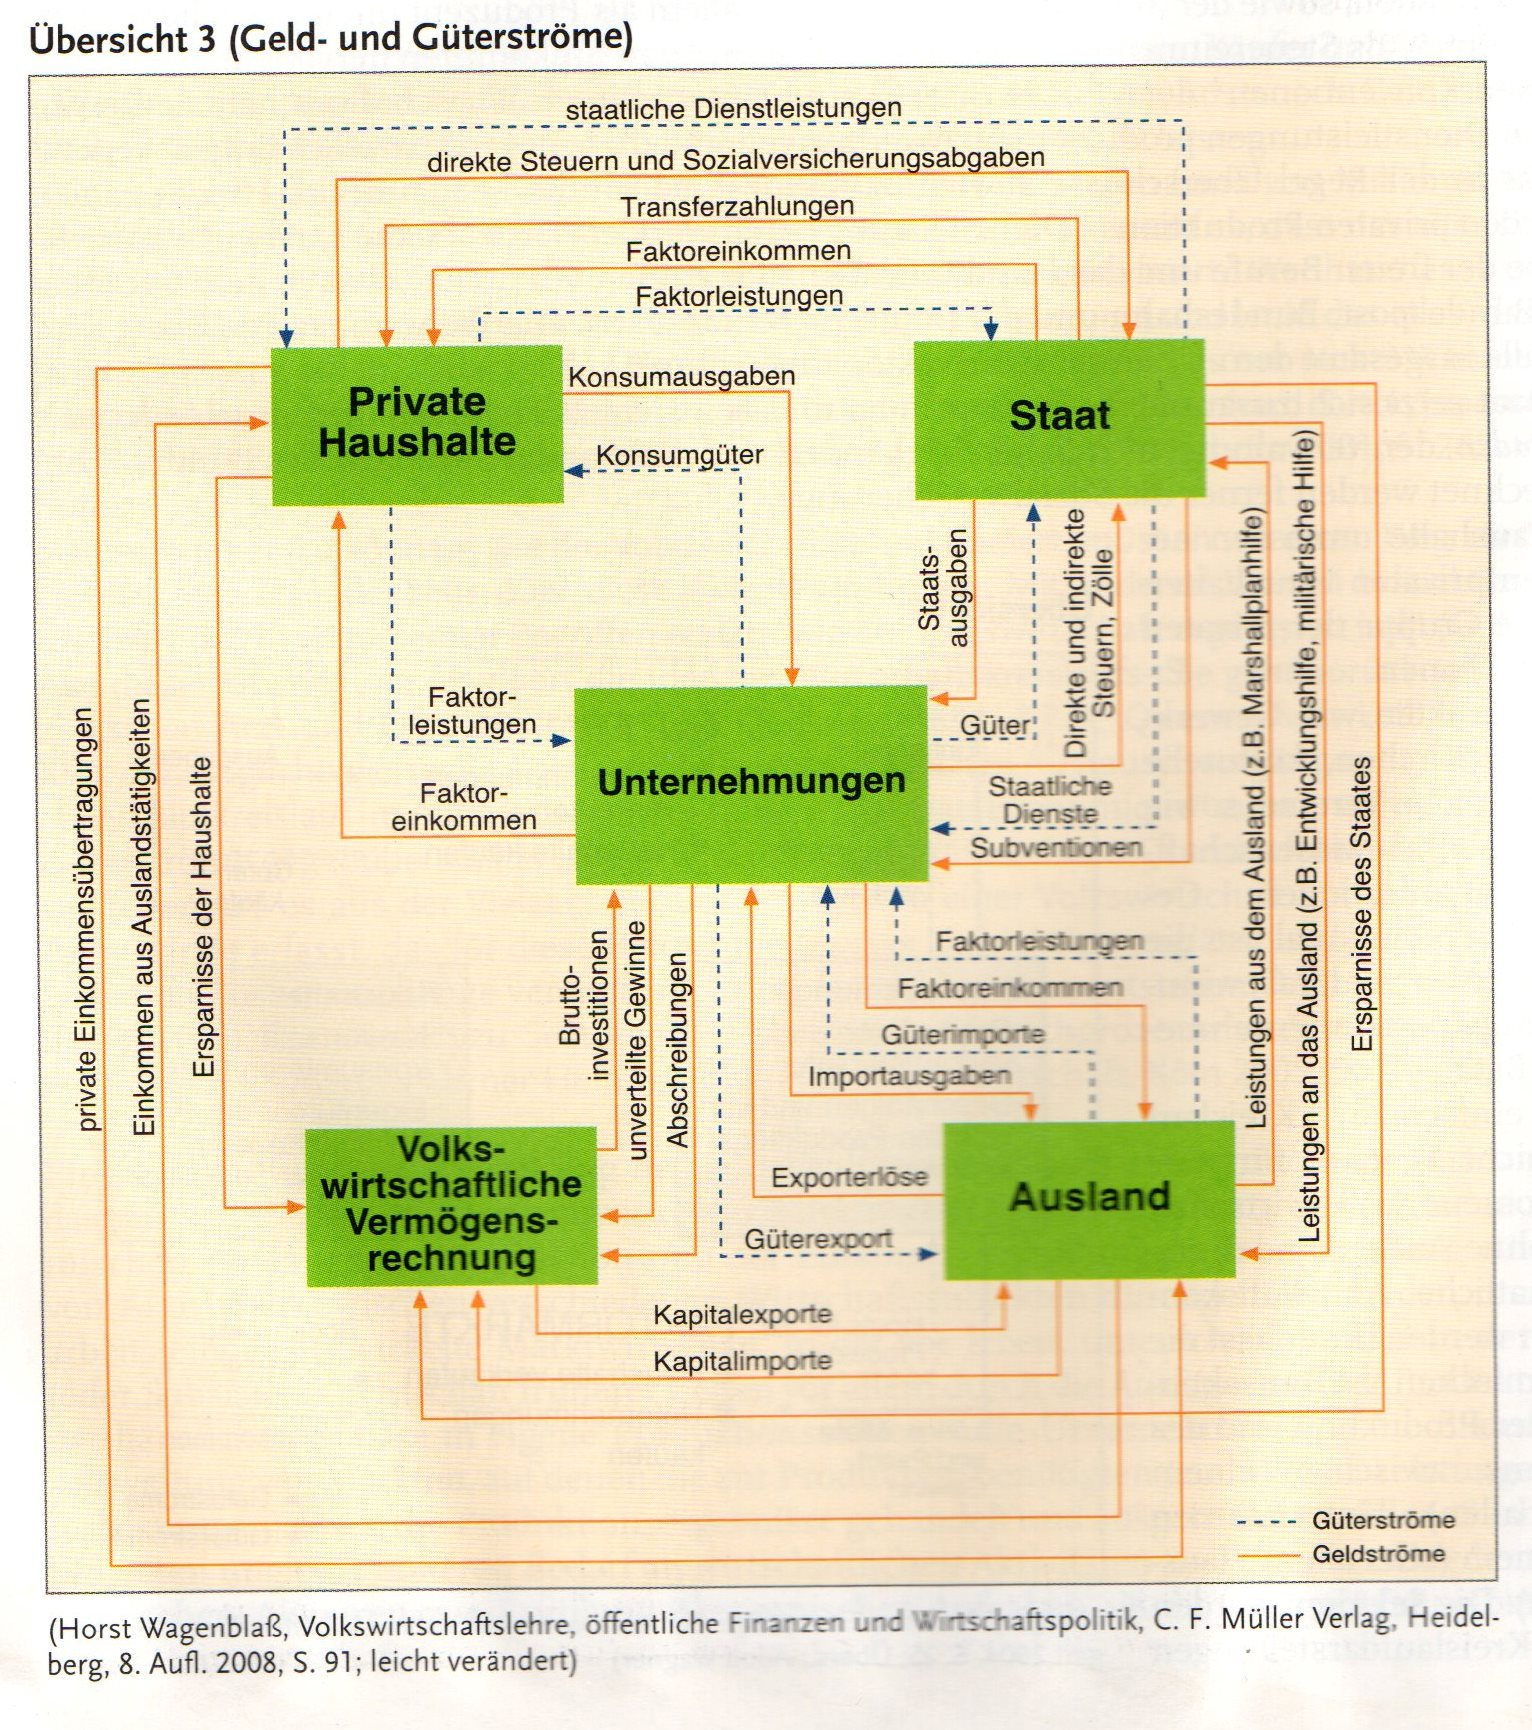
\includegraphics[scale=1.0]{pictures/lf01-pic/lf01-wirtschaftskreislauf.jpg}

%%% Ende: Wirtschaftskreislauf
%%%%%%%%%%%%%%%%%%%%%%%%%%%%%%%%%%%%%%%%%%%%%%%%%%%%%%%%%%%%%%%%%%%%%%%%%%%%%%%%

%%% Anfang: Marktstrukturen und ihre Auswirkungen
\subsection{Marktstrukturen und ihre Auswirkungen}

Was ist ein Markt? Märkte sind Orte, an denen Angebot und Nachfrage aufeinandertreffen und durch den Ausgleich von Angebot und Nachfrage bildet sich ein Preis. Es gibt verschiedene Arten von Märkten, zum einen Faktormärkte -- bspw. Arbeitsmarkt -- und zum anderen Gütermärkte. Daneben gibt es noch verschieden Marktformen:\\
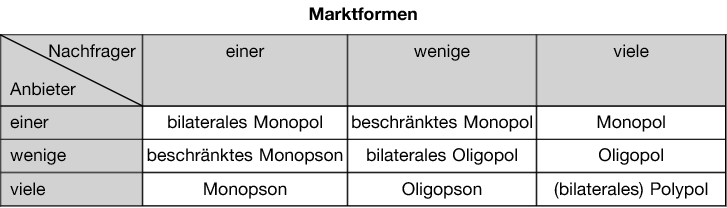
\includegraphics[scale=0.6]{pictures/lf01-pic/lf01-marktformen.png}

\subsubsection{Anbieter- und Nachfragerverhalten}
Das Verhalten von Anbietern und Nachfragern stellen Einflussfaktoren auf den Märkten dar.

{\bf Einflussfaktoren auf Seiten der Anbieter:}
\begin{itemize}
	\item Kosten der Produktionsfaktoren
	\item Gewinnerwartung
	\item Preis des Angebots
	\item Preis der Konkurrenz
	\item Stand der technischen Entwicklung
\end{itemize}

{\bf Einflussfaktoren auf Seiten der Nachfrager: }
\begin{itemize}
	\item Art und Dringlichkeit der Nachfrage
	\item Preis des nachfragten Gutes
	\item Preise der Konkurrenz
	\item Höhe der Kaufkraft
	\item Zukunftserwartungen der Konsumenten
\end{itemize}

Bei dem vollkommenen Markt handelt es sich um eine theoretische Vereinfachung der Realität. Der vollkommene Markt erfüllt folgende Bedingungen:

\begin{itemize}
	\item Rationales Verhalten aller Teilnehmer
	\item Homogenität aller Güter
	\item Keine Präferenzen der Teilnehmer
	\item Vollständige Markttransparenz
	\item Unendliche Reaktionsgeschwindigkeit der Teilnehmer
\end{itemize}

Durch diese Optimalisierung der Realität gibt es nahezu nur unvollkommene Märkte. Dem vollkommenen Markt am nächsten kommt die Börse. \\

Unter den Annahmen, dass vollständige Konkurrenz herrscht und dass Angebot und Nachfrage bloß vom Preis abhängen, gilt: (1) Wenn der Preis steigt, sinkt die Nachfrage \& (2) Wenn der Preis steigt, dann steigt das Angebot.\\

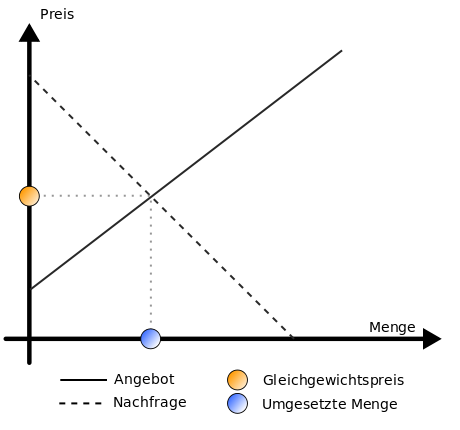
\includegraphics[scale=0.7]{pictures/lf01-pic/lf01-gleichgewichtspreis.png}\\
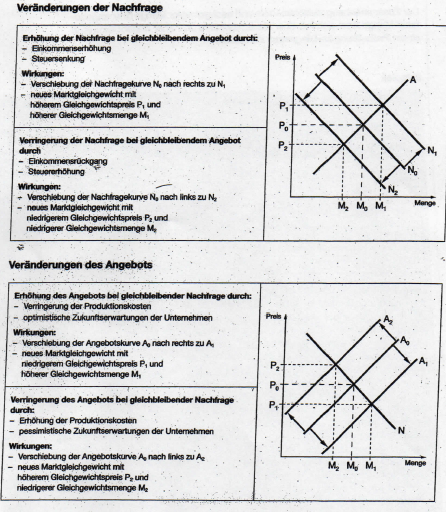
\includegraphics[scale=1.0]{pictures/lf01-pic/lf01-nachfrageverschiebung.png}
%%% Ende: Marktsturkturen und ihre Auswirkungen
%%%%%%%%%%%%%%%%%%%%%%%%%%%%%%%%%%%%%%%%%%%%%%%%%%%%%%%%%%%%%%%%%%%%%%%%%%%%%%%%

%%% Anfang: Kooperation \& Konzentration
\subsection{Kooperation \& Konzentration}

\begin{itemize}
	\item horizontale Kooperation
		\begin{itemize}
			\item Unternehmen gleicher Wirtschaftsstufe
			\item gleichartige Güter werden produziert
		\end{itemize}
	\item vertikale Kooperation
		\begin{itemize}
			\item Unternehmen unterschiedlicher Wirtschaftsstufen
		\end{itemize}
	\item anorganische Kooperation
		\begin{itemize}
			\item Unternehmen unterschiedlicher Wirtschaftsstufen und Branchen
		\end{itemize}
\end{itemize}

\begin{itemize}
	\item horizontale Konzentration
		\begin{itemize}
			\item Unternehmen gleicher Wirtschaftsstufe und Branche fusionieren zu einem Unternehmen
		\end{itemize}
	\item vertikale Konzentration
		\begin{itemize}
			\item Unternehmen unterschiedlicher Wirtschaftsstufen und gleicher Branche fusionieren zu einem Unternehmen
			\item Ein größerer Teil der Produktionskette kann von dem neuen Unternehemen verwirklicht werden
		\end{itemize}
	\item diagonale Konzentration
		\begin{itemize}
			\item Unternehmen unterschiedlicher Wirtschaftsstufen und Branchen fusionieren zu einem Unternehmen
			\item Ein Mischkonzern entsteht
			\item Es wird für Risikosträuung gesorgt
		\end{itemize}
\end{itemize}


\subsection{Entgeltabrechnung}

\subsubsection{Gehaltsbestandteile} 
Das Gehalt kann sich aus mehreren Faktoren zusammensetzen:
\begin{itemize}
	\item Grundlohn
	\item Naturallohn
		\begin{itemize}
			\item z.B. zusätzlich bei der Seeschiffahrt, im Nahrungsmittelbereich als "freie Kost und Logis"
		\end{itemize}
	\item Zeitlohn
		\begin{itemize}
			\item Bezahlung auf Basis der geleisteten Arbeitszeit
		\end{itemize}
	\item Zuschlag
		\begin{itemize}
			\item Zuschläge für besondere Leistungen oder Belastungen des Arbeitsnehmers
			\item z.B. überstunden, Nachtarbeit, Spätschicht, Schmutzzuschlag, Hitzezuschlag, Kinderzuschlag, Ortszuschlag, Leistungszuschlag
		\end{itemize}
	\item Akkordlohn
		\begin{itemize}
			\item Bezahlung nach geleistetem Arbeitsergebnis unabhängig von der Arbeitszeit
		\end{itemize}
	\item Prämiensystem
		\begin{itemize}
			\item Zeitlohn und zusätzlich entsprechend der Leistung eine Prämie
		\end{itemize}
	\item Provision
		\begin{itemize}
			 \item Prozentuale Beteiligung am Wert der eigenen Geschäfte
		\end{itemize}
	\item Gratifikation
		\begin{itemize}
			\item Sonderzuwendung bei besonderen Anlässen
			\item z.B. Weihnachten, Jubiläum, Erreichung eines besonderen Ziels
		\end{itemize}
	\item Gewinnbeteiligung
		\begin{itemize}
			\item Beteiligung am Geschätsergebnis des Unternehmens
		\end{itemize}
	\item Vermögenswirksame Leistungen
		\begin{itemize}
			\item Ein Teil des Arbeitsverdienstes wird vermögenswirksam angelegt
			\item Arbeitgeber kann sich durch individuelle Vereinbarungen an den Beiträgen beteiligen
		\end{itemize}
	\item Aufwendungsersatz
		\begin{itemize}
			\item Aufwendungen des Arbeitnehmers müssen ersetzt werden
			\item z.B. Reisespesen oder Auslagen zur Beschaffung von Werkzeugen
		\end{itemize}
\end{itemize}

\subsubsection{Abzüge}
Faktoren, die sich auf die Gehaltsabrechnung auswirken:
\begin{itemize}
	\item Einkommenshöhe
		\begin{itemize}
			\item Die Lohnsteuer wird nur auf den Einkommensanteil oberhalb des Grundfreibetrages erhoben
		\end{itemize}
	\item Familienstand: Steuerklasse
	\item Kirchenmitgliedschaft
		\begin{itemize}
			\item Kirchensteuer
		\end{itemize}
	\item Krankenkasse
		\begin{itemize}
			\item Variable Zusatzbeiträge
		\end{itemize}
	\item Wohnort
		\begin{itemize}
			\item Solidaritätszuschlag
			\item Kirchensteuersatz
		\end{itemize}
\end{itemize}

Die Beiträge zur Sozialversicherung werden zur Hälfte vom Arbeitgeber getragen:
\begin{itemize}
	\item Rentenversicherung (19,9\%)
	\item Pflegeversicherung (1,7\% + 0,25\% für Kinderlose ab einem Alter von 23 Jahren)
	\item Arbeitslosigkeit (4,2\%)
	\item Krankenkasse (variabel + 0,9\% Zusatzbeitrag für Arbeitnehmer)
\end{itemize}
Bei Azubis mit einem Gehalt unter 325\euro brutto übernimmt der Arbeitgeber die Versicherungsbeiträge vollständig.

Weiter Abzüge: Lohnsteuer, Solidaritätsbeitrag, Kirchensteuer

Lohnsteuerklassen:
\begin{itemize}
	\item Klasse I: ledig, geschieden, verwitwet
	\item Klasse II: Steuerklasse I mit min. einem Kind
	\item Klasse III: verheiratet, ein Verdiener
	\item Klasse IV: verheiratet, zwei Verdiener in IV, beide Verdienen etwa gleich viel
	\item Klasse V: verheiratet, zwei Verdiener, Partner in III, Verdienst ist unterschiedlich
	\item Klasse VI: mehrere Lohnsteuerkarten
\end{itemize}

\subsubsection{Beispielabrechnung}
Voraussetzungen: Angestellte, ledig, 24 Jahre, 2.100\euro brutto, Lohnsteuer: 287,33\euro , Kirchensteuersatz 9\%, Solidaritätszuschlag: 5,5\% Beitragssatz zur Krankenkasse: allgemeiner Beitragssatz: 13,8\%, zusätzlicher Beitragssatz: 0,9\%, Beitragssatz zur Rentenversicherung: 19,5\%
Beitragssatz zur Arbeitslosenversicherung: 4,5\%, Beitragssatz zur Pflegeversicherung: 1,7\% \\
\\
$Kirchensteuer = Lohnsteuer * Kirchensteuersatz = 287,33\textit{\euro} * 9\% = 25,85\textit{\euro}$\\
$Solidaritätszuschlag = Lohnsteuer * 5,5\% = 287,33\textit{\euro} * 5,5\% = 15,80\textbf{\euro}$\\
$Krankenversicherung = \frac{Bruttolohn * Krankenversicherungssatz}{2} + Bruttolohn * Zusatzbeitrag = \frac{2100\textit{\euro} * 13,8\%}{2}+2100\textit{\euro} * 9\% = 163,80\textit{\euro}$\\
$Rentenversicherung = \frac{Bruttolohn * Rentenversicherungssatz}{2} = \frac{2100\textit{\euro}}{2} = 204,75\textit{\euro}$\\
$Arbeitslosenversicherung = \frac{Bruttolohn * Arbeitslosenversicherungssatz}{2} = \frac{2100\textit{\euro}* 4,5\%}{2} = 47,25\textit{\euro}$\\
$Pflegeversicherung = \frac{Bruttolohn * Pflegeversicherungssatz}{2} + Bruttolohn * Zusatzbeitrag = \frac{2100\textit{\euro} * 1,7\%}{2} + 2100\textit{\euro} * 0,25\% = 23,10\textit{\euro}$\\
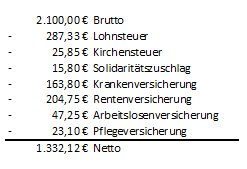
\includegraphics[scale=1.0]{pictures/lf01-pic/lf01-beispielentgeldabrechung.png}


\subsection{Rechts- und Geschäftsfähigkeit}

Wichtige Punkte, die in einem Kaufvertrag notiert werden sollten:
\begin{itemize}
	\item Art und Güte der Leistung
	\item Lieferzeit
	\item Verpackungs- und Versandkosten
	\item Zahlungsart
	\item Preis
	\item Erfüllungsort
\end{itemize}

\subsubsection{Rechtsordnung}
Die Rechtsordnung unterscheidet zwischen dem öffentlichen und dem Privaten Recht.\\
Das {\it öffentliche Recht} beschreibt die Rechtsbeziehungen zwischen den Einzelpersonen und dem Staat. Dies ist z. B. im Steuerrecht und im Strafrecht der Fall.\\
Das {\it Private Recht} beschreibt die Rechtsbeziehungen zwischen den Einzelpersonen, wie es z. B. im BGB und im HGB der Fall ist.\\
\\
\begin{itemize}
	\item Rechtsfähigkeit
		\begin{itemize}
			\item Fähigkeit, Träger von Rechten und Pflichten zu sein
			\item Natürliche Personen
				\begin{itemize}
					\item Menschen von Geburt bis Tod
				\end{itemize}
			\item Juristische Personen
				\begin{itemize}
					\item Vereine
					\item Stiftungen
					\item Handelsgesellschaften mit Eintragung in das jeweilige Register (z.B. GmbH, AG)
				\end{itemize}
		\end{itemize}
	\item Geschäftsfähigkeit
		\begin{itemize}
			\item Fähigkeit, selbstständig und wirksam Rechtsgeschäfte abschließen zu können
			\item geschäftsunfähig (Willenserklärungen sind nichtig)
				\begin{itemize}
					\item Kinder bis zum vollendeten 7. Lebensjahr
					\item geschäftsunfähige Personen (§ 104 BGB)
					\item {\it Ausnahmen:} volljährige Geschäftsunfähige, die Geschäfte des täglichen Lebens mit geringen Mitteln bewirken (§ 105 BGB)
				\end{itemize}
			\item beschränkt geschäftsfähig (Willenserklärungen sind schwebend unwirksam)
				\begin{itemize}
					\item Kinder zwischen dem vollendeten 7. und vollendetem 18. Lebensjahr (§§ 106 bis 113 BGB)
					\item betreute Volljährige mit gerichtlichem Einwilligungsvorbehalt für bestimmte Handlungsbereiche. {\it Hinweis:} Der gesetzliche Vertreter kann auch nachträglich genehmeigen.
					\item Taschengeldgeschäfte nach § 110 BGB
					\item vorteilhafte Rechtsgeschäfte nach § 107 BGB
					\item selbstständiger Betrieb eines Erwerbsgeschäftes nach § 112 BGB
					\item genehmigte Arbeitsverhältnisse nach § 113 BGB
				\end{itemize}
			\item voll geschäftsfähig 
				\begin{itemize}
					\item alle sonstigen volljährigen Personen
				\end{itemize}
		\end{itemize}
	\item Deliktfähigkeit (vgl. § 828 BGB) / Schuldfähigkeit (vgl. § 19 StGB)
		\begin{itemize}
			\item Verantwortung für unerlaubte Handlungen (Aufsichtspflicht beachten)
		    \item deliktunfähig
		    	\begin{itemize}
		    		\item Kinder bis zur Vollendung des 7. Lebensjahres
		    	\end{itemize}
		    \item beschränkt deliktfähig
		    	\begin{itemize}
		    		\item Minderjährige zwischen 7 und 18 Jahren und Taubstumme (Schuldfähigkeit ab 14 Jahren)
		     	\end{itemize}
		     \item voll deliktfähig
		     	\begin{itemize}
		     		\item Personen ab Vollendung des 18. Lebensjahres, sofern geschäftsfähig
		     	\end{itemize}
		\end{itemize}
	
\end{itemize}
\subsubsection{Rechtsgeschäfte}

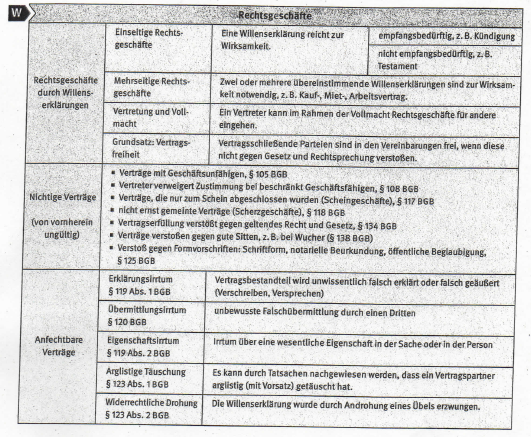
\includegraphics[scale=1.3]{pictures/lf01-pic/lf01-rechtsgeschaefte.png} 


%\section{Lernfeld 1B - Recht und Wirtschaft}

Im Lernfeld 1B \ql Recht und Wirtschaft\qr\ werden die rechtlichen Rahmenbedingungen des Wirtschaftens besprochen. Zu den Themen gehören unter anderem Rechtssubjekte, -objekte und -geschäfte.


%%% Rechtssubjekte
% natürliche und juristische Personen, Geschäftsfähigkeit


%%% Rechtsobjekte


%%% Rechtsgeschäfte
% Arten und Formen, Nichtigkeit und Anfechtbarkeit, Vertragsarten, Störungen
%\section{Lernfeld 2 - Geschäftsprozesse und betriebliche Organisation}

\subsection{Projektmanagment}

Kriterien eines Projektes:
\begin{itemize}
	\item Einmaligkeit
	\item Zeitbegrenzung
	\item Bedeutsamkeit
	\item Komplexität
	\item Fachübergreifend
	\item Risiko
\end{itemize}

Anlässe für Projekte: Bsp.
\begin{itemize}
	\item Organisatorische Probleme: schlechter Informationsfluss
	\item Technische Probleme: hoher Wartungsaufwand
	\item Wirtschaftliche Probleme: sinkende Umsätze
	\item Marktbezogene Entwicklungen: Wettbewerbsdruck
	\item Innovation: neue Produktideen
	\item Controlling-Ergebnisse: ineffiziente Systeme
\end{itemize}

Magisches Dreieck des Projektmanagments:\\
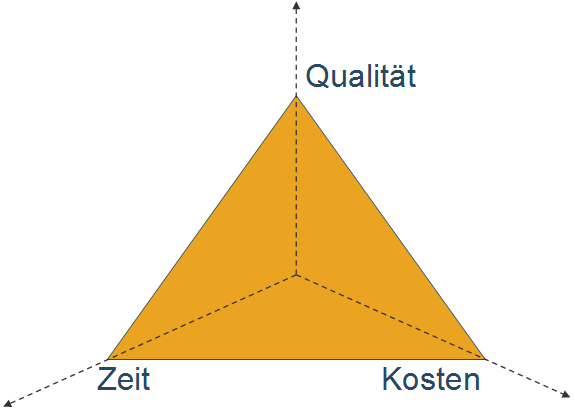
\includegraphics[scale=0.5]{pictures/lf02-pic/lf02-projekt-dreieck.png}

Wenn ein \textbf{Projektantrag} genehmigt wird, wird daraus ein \textbf{Projektauftrag}. Der Projektantrag enthält folgende Informationen:
\begin{itemize}
	 \item Aufgabenbeschreibung
	 \item Erwarteter Nutzen
	 \item Konsequenzen bei Nicht-Beachtung
	 \item Rahmenbedingungen
\end{itemize}
Projektauftrag:
\begin{itemize}
	\item Was soll realisiert werden?
	\item Welche Qualität wird angestrebt?
	\item Wie viel soll realisiert werden?
	\item Personal: wer wird eingesetzt?
	\item Material: womit wird die Realisierung erfolgen?
	\item Zeitrahmen: wie lange soll das Projekt dauern?
	\item Wo soll das Projekt umgesetzt werden?
	\item Welche Risiken bestehen?
\end{itemize}

\begin{itemize}
	\item Minimalprinzip
	\item Maximalprinzip
\end{itemize}


\subsection{Motivation}
- Herzberg
- Maslow

\subsection{Projektcontrolling}
\subsubsection{Balanced Scorecard}
%\section{Lernfeld 4 - Einfache IT-Systeme (Oenings und Wächter)}
%

\subsection{Software-Klassifikation}
eCl@ss

\subsection{Interrupts}
Beispielsweise einmal pro Sekunde wird nach einem Interrupt geschaut. Es gibt aber auch Algorithmen, die nach jedem Befehl nach einem Interrupt.

Wenn ein Interrupt durchkommt, wird der Interrupt mit einer Bibliothek abgeglichen, 

Interrupts: hardware-, softwarebedingte und direct memory access (DMA).

Ursachen für Interrupts
\begin{itemize}
	\item Fehlersituation: Fehler bei Rechenoperationen (bspw. Div. durch Null)
	\item Software-Interrupt: bspw. {\it kill}
	\item Hardware-Interrupt: Periperieeinheiten meldet über ein Signal ein Ereignis an die Software.
\end{itemize}

Interruptvektor

Systemstapel
Unterbrechungsroutine
Benutzerprogramm

Programmzähler
Register
Stapelzeiger

Insgesamt läuft eine Unterbrechung, die durch ein E/A-Gerät ausgelöst wurde in folgenden Schritten ab:
\begin{enumerate}
	\item Der Controller des E/A-Ger̈ats sendet ein Signal.
	\item Nach Ausführung des aktuellen Befehls wird das laufenden Programm unterbrochen.
	\item Die CPU analysiert die aufgetretene Unterbrechung.
	\item Der Zustand des unterbrochenen Programms wird gerettet.
	\item Die Unterbrechungsroutine wird ausgeführt.
	\item Der Zustand des unterbrochenen Programms wird wiederhergestellt, und es wird fortgesetzt.
\end{enumerate}


Synchrone Unterbrechungen. Wahrscheinlichkeit des Auftretens (WSK).
\begin{itemize}
	\item Software-Interrupts durch Trap-Befehle (WSK=1)
	\item Division durch Null, Überlauf usw. (WSK datenabhängig)
	\item Trace-Unterbrechung (WSK=1)	
\end{itemize}
Asynchrone Unterbrechungen
\begin{itemize}
	\item Busfehler (WSK hardware- und umgebungsabhängig)
	\item Unterbrechungen ausgelöst von Peripherieeinheiten (WSK peripherieabhängig)
\end{itemize}

Unterbrechungsvektor ist eine Zuordnungstabelle der Interrupts zu den entsprechenden Interrupt-Routinen im RAM.

Maskierung: Bit-Maske, bspw. Netzwerkmasken (255.255.255.0 oder Präfixe /24)

Unterbrechungskontext

%
\subsection{Prozessmanagment (Scheduling)}


Central Processing Units (CPUs) können trotz Hyperthreading und mehreren Kernen trotzdem nur einen Befehl gleichzeitig ausführen. Damit gleichzeitig mehrere Programme laufen können, muss festgelegt werden, welches Programm wann wie viel Prozessor-Zeit beanspruchen darf. Der Teil des Betriebssystem, der diese Zuteilung kontrolliert, wird Schedular genannt. Wie genau der Schedular die Zeit verteilt, legt der sogenannte Scheduling Algorithmus fest. Das eigentliche Einspielen des Prozesses wird vom Dispatcher umgesetzt. 

Ein Programm besteht aus dem Code, den zu bearbeitenden Daten und dem Stack. Ein Prozess ist ein Programm in Ausführung und besteht aus Programmdaten und dem Prozesskontext. Prozesse müssen in verschiedenen Situationen auf bestimmte Ereignisse warten, bspw. das Laden von Daten. In dieser Wartezeit werden dann andere Prozesse berechnet.

Im RAM liegen verschiedene Daten der Prozesse. Im sogenannten Programmsegment liegen der ausführbare Code des Programms. Im Datensegment liegen die Daten, die ein Prozess bearbeitet.

Alle Daten, die das Betriebssystem über einen Prozess verwalten muss,bezeichnet man als Prozesskontrollblock (PCB), und alle PCBs zusammen werden in einer Prozesstabelle organisiert. Im Prozesskontrollblock stehen insbesondere folgende Informationen:
\begin{itemize}
	\item Prozessidentifikation: Jeder Prozess erhält eine ID zur eindeutigen Identifizierung
	\item Prozessorstatus: Enthält die Informationen über den Zustand des Programms, in dem es fortgesetzt werden soll
	\item Prozeskontrollinformationen: Priorität des Prozesses, Informationen über den Speicherbereich, geöffnete Dateien des Prozesses \dots
\end{itemize}

\subsubsection{Scheduling-Algorithmen: Varianten}

Prinzipiell gibt es zwei Arten: (1) \textbf{Nicht preemptives Scheduling} und (2) \textbf{preemtives Scheduling}. Ersteres ist nicht interaktiv und wird bei Stapelverarbeitungssystemen benutzt. Befindet sich ein Prozess im Zustand \ql running\qr, so wird seine Ausführung solange fortgesetzt, bis er terminiert oder durch Warten auf Ressourcen blockiert. Letzter lassen die Unterbrechung von Prozessen zu, sodass eine Interaktion möglich wird. Dadurch geht der Prozess in den Zustand \ql ready\qr\ über.

Die Anforderungen an einen Scheduling-Alorithmus hängen stark davon ab, welche Aufgaben ein System zu erfüllen hat. Je nach Aufgabe lässt sich so der Algorithmus optimieren.

Zu den Anforderungen an alle Algorithmen gehören die Faktoren \textbf{Fairness}, \textbf{Policy Enforcement}, \textbf{Balance}, \textbf{Datensicherheit}, \textbf{Skalierbarkeit} und \textbf{Effizienz}. Das bedeutet beispielsweise, dass jeder Prozess einen gerechten Anteil an der Prozessor-Zeit erhält und auch, dass jeder Prozess eine endliche Zeit warten muss. Weitere Anforderungen werden in nutzer- und systemorientierte Kriterien geteilt. Nutzerorientierte Kriterien spielen vor allem in interaktiven Systemen eine Rolle, wohingegen systemorientierte Kriterien in Echtzeitsystemem\footnote{In Echtzeitsystemen muss gewährleistet werden, dass ein bestimmter Prozess zu einer bestimmten Zeit berechnet wurde. Bei Nicht-Echtzeitsystemen ist nicht vorhersehbar, wann ein bestimmter Prozess abgeschlossen sein wird. Daher werden Echtzeitsysteme vor allem in kritischen Umgebungen verwendet, bspw. in embedded-systems} im Vordergrund stehen.
\begin{itemize}
 \item Stapelverarbeitungssysteme: Durchsatz soll maximiert werden, Minimierung der Verweildauer, Konstante/maximale CPU-Auslastung
 \item Interaktive Systeme: Antwortzeit sollte minimal sein, Verhältnismäßigkeit der Antwortzeiten, Anzahl der Interaktionen sollte maximal sein können
 \item Echtzeitsysteme: Sollzeitpunkt, Vorhersagbarkeit
\end{itemize}

\subsubsection{Nicht-preemptive Scheduling-Algorithmen: Stapelverarbeitungssysteme}

Stapelverarbeitungssysteme sind etwa alte Lochkarten-Maschinen. Dabei ist im Gegensatz zu interaktiven Systemen nach dem Starten des Prozess kein Eingreifen durch den Nutzer vorgesehen.

\textbf{First-Come-First-Serve} (FCFS) ist der einfachste aller Scheduling-Algorithmen, jedoch sind keine Unterbrechungen vorgesehen. D.h., ein Prozess läuft solange, bis er fertig ist. Dazwischen kann kein anderer Prozess auf die CPU zurückgreifen.

Der Algorithmus \textbf{Shortest-Job-First} (SJF) geht davon aus, dass die Laufzeit der Prozesse vorher bekannt ist. SJF wählt immer den Prozess zuerst, der am kürzesten ist.

\textbf{Shortest Remaining Time Next} (STRN) wählt, wie der Name bereits zeigt, den Prozess, der die niedrigste verbleibende Laufzeit besitzt.

\subsubsection{Preemptive Scheduling-Algorithmen: interaktive Systeme}

\textbf{Round-Robin Scheduling} (RRS) ist der älteste und einfachste Algorithmus für interaktive Systeme. Dabei erhält jeder Prozess abwechselnd einen gleich großen Zeitabschnitt (sog. Quantum). Das Verfahren wird auch Zeitscheibenverfahren oder Time-Sharing genannt.

\textbf{Prioritätsbasiertes Scheduling}. Wie wir bereits wissen, können Prozessen eine Priorität zugeordnet werden. Unter Linux wird die Priorität von dem sogenannten Nice-Wert repräsentiert. Beim RRS wird hingegen angenommen, dass alle Prozesse gleich wichtig sind.

Damit ein Prozess mit niedriger Priorität nicht immer wieder aufgeschoben wird, kann der Algorithmus beispielsweise bei jedem Takt den Wert die Priorität erhöhen.

\textbf{Multilevel Feedback Queueing} (MLFQ): Das besondere dieses Algorithmus ist - im Gegensatz zu SPN und SRPT - dass man keine Kenntnisse über die voraussichtliche Abarbeitungszeit braucht und trotzdem kurze Aufträge bevorzugen kann. Das Scheduling wird nun unterbrechend ausgeführt; Prioritäten werden dabei dynamisch vergeben.


\subsection{Lizenzen}
\subsubsection{Open Source}

Open Source nennt man Software, deren Lizenzbestimmungen in Bezug auf die Weitergabe der Software besagen, dass der Quelltext {\it öffentlich} zugänglich sein muss. Abhängig von der jeweiligen Lizenz kann diese unter Umständen auch beinhalten, dass die Software frei kopiert, modifiziert und verändert wie unverändert weiterverbreitet werden darf.

Open-Source-Software (OSS) steht unter einer der von der Open Source Initiative (OSI) anerkannten Lizenzen. Die OSI verwendet dabei den Begriff Open Source auf all die Software an, deren Lizenzverträge den folgenden drei Merkmalen entsprechen und die zehn Punkte der Open Source Definition erfüllen:
\begin{enumerate}
	\item Die Software (d. h. der Quelltext) liegt in einer für den Menschen lesbaren und verständlichen Form vor.
	\item Die Software darf beliebig kopiert, verbreitet und genutzt werden.
	\item Die Software darf verändert und in der veränderten Form weitergegeben werden.
\end{enumerate}

Ein frühes und bekanntes Beispiel für OSS ist Mozillas Firefox. Dieser entstand 2002 aus der Freigabe des Quelltextes des Netscape Navigators im Jahre 1998.

Zu beachten ist, dass Open Source Software im frei im Sinne von Freiheit ({\it free speech, not free beer}) ist und nicht im Sinne von kostenlos. Um Missverständnissen vorzubeugen wird sie daher {\it open} statt {\it free} genannt. Aber auch diese Regelung ist nicht unproblematisch. Beispielsweise kritisiert die Free Software Foundation (FSF) vor allem die Tatsache, dass der Begriff Open Source die Einsicht in den Quellcode einer Software hervorhebt, nicht aber die Freiheit, diesen Quellcode auch beliebig weiterzugeben oder zu verändern. Die PGP Corporation bezeichnet zwar PGP als Open Source, weil der Quellcode gegen eine Gebühr einsehbar ist, jedoch darf er weder verändert oder weitergegeben werden.

\subsubsection{Freeware}

Freeware bezeichnet im allgemeinen Sprachgebrauch Software, die vom Urheber zur kostenlosen Nutzung zur Verfügung gestellt wird. Freeware ist meistens proprietär und steht damit laut der Free Software Foundation im Gegensatz zu Freier Software, die weitläufigere Freiheiten, wie Veränderungen an der Software, gewährt.

\subsubsection{Commercial Software}
Commercial Software, oder auch Payware, ist Software, die für den Verkauf bestimmt ist. Kommerzielle Software kann sowohl properitär als auch unter free/open source Software sein.
%
\subsection{Boot-Prozess}
Beim Bootstrapping (Bootstrap-Prozess) wird der Bootloader (bspw. GRUB) aus dem Master Boot Record (MBR) gelesen und in den RAM geschrieben. Der MBR liegt im ersten Sektor der Festplatte/SSD. Der Bootloader lädt dann den Kernel in den RAM (s. Memory Mangament).

Der Ablauf ist wie folgt: BIOS -> POST -> INT -> BOOT -> HW Check -> Kernel

\subsubsection{BIOS vs UEFI}
Als Nachfolger des BIOS kommt langsam das UEFI durch. Dieses bietet viele Möglichkeiten, die auf System mit klassischem BIOS erst nach dem Laden des Betriebssystems möglich waren. Eine wichtige Neuerung ist der Secure-Boot Modus, mit dem nur vorher signierte Bootloader verwendet werden können. So wird das Risiko eine Infektion mit Schadsoftware über manipulierte Bootloader minimiert. Zusätzlich bietet UEFI die Möglichkeit einer Netzwerkverbindung ohne geladenem Betriebssystem. So kann zum Beipiel Fernwartung schon im Bootprozess ansetzen. Das UEFI ist durch die Nutzung der Grafikfähigkeit aktueller Hardware viel einfacher zu Bedienen als das klassische BIOS: Das UEFI ist außerdem dazu in der Lage, dass Treiber bereits darin eingearbeitet werden und so systemunabhängig verwendet werden. In Zukunft lassen sich auch speziell für das UEFI geschriebene Anwendungen schon vor dem Laden des Betriebssystems nutzen. So könnten viele einfache Anwendungen schon bald ohne zeitaufwändigen Bootvorgang verwendet werden.

Durch die Verwendung von GPT statt MBR ist es möglich, Festplatten >2TB zu nutzen.

Die Kritik an UEFI gründet in erster Linie auf der Komplexität, da UEFI fast schon ein eigenes Betriebssystem darstellt.

\subsubsection{Power On Self-Test (POST)}
Der Power-On-Self-Test (POST) ist der erste Schritt des Bootvorgangs. In diesem Schritt führt der Prozessor die ersten Programmanweisungen des BIOS aus. Diese beinhalten einen Test, der überprüft, ob die notwendigen Geräte angeschlossen und auch funktionsfähig sind.  Teilweise werden auch schon Informationen ausgewertet, welche im CMOS-Speicher auf der Hauptplatine abgelegt sind. In dieser Phase können nur hardwarebedingte Fehler auftreten, da das Betriebssystem erst später geladen wird.  Diese wären z.B. ein defekter Arbeitsspeicher oder falsch montierte Verbindungskabel.  Ansonsten können aus fehlerhafte Einstellungen im BIOS-Setup zu Fehlern führen. Dies kann z.B. durch einen Datenverlust im CMOS-Speicher vorkommen.

\subsubsection{Initiale Startphase}
Die Initiale Startphase ist die zweite Phase des Bootvorgangs und startet, nachdem der POST erfolgreich abgeschlossen wurde. Nun werden die Laufwerke nach der im BIOS eingestellten Reihenfolge nach einem Betriebssystem gefunden. Ist dieses gefunden, so wird der Bootsektor des Betriebssystems in den RAM geladen.

Ein wichtiger Risikofaktor ist dabei jedoch, dass der in diesem Bootsektor enthaltene Programmcode unabhängig vom Inhalt geladen und ausgeführt wird.  So können an dieser Stelle Bootsektorviren ansetzten, die den restlichen Virencode dann danach nachladen können. Wenn der Virus vom Bootmedium in den Arbeitsspeicher geladen wurde, kann er sich auch auf der Festplatte einnisten, um im weiteren Verlauf bei jedem Systemstart präsent zu sein.

Ist als Bootlaufwerk die primäre Festplatte des Computers gefunden, wir zuerst der Masterbootsektor (MBR) geladen. Der MBR enthält die Partitionstabelle, welche die Informationen über die Aufteilung der Festplatte in einzelne Partitionen enthält, und den MBR-Code, welcher umgehend ausgeführt wird.  Aus der Partitionstabelle ermittelt der MBR-Code die aktive primäre Partition. Aus dieser wird der betriebssystemabhängige Bootsektorcode geladen und ausgeführt.

\subsubsection{Bootloader-Phase}
Zunächst wird die CPU aus dem Real-Modus in den Protected-Modus umgeschaltet, damit der gesamte Arbeitsspeicher genutzt werden kann. Der Bootloader enthält bereits die notwendigen Routinen, um Datenträger, die in NTFS, FAT 16 oder FT 32 formatiert sind, lesen bzw. zu beschreiben. Nach diesem Schritt wird die Datei BOOT.INI aus dem Startlaufwerk analysiert. Wenn nur ein Betriebssystem in dieser Datei verzeichnet ist, so wird umgehend die Hardware-Erkennungs-Phase eingeleitet. Sind jedoch mehrere Systeme verzeichnet, so erscheint ein Auswahlmenü, in dem der Benutzer die gewünschte Installation auswählen kann. Wird in einer vordefinierten Zeit keine Auswahl getroffen, so wird die in der BOOT.INI eingetragene Standardinstallation gestartet. Diese Einstellungen lassen sich auch in der BOOT.INI Datei verändern.

\subsubsection{Hardware-Erkennungs- und Konfigurations-Phase}
In der Hardware Erkennungs- und Konfigurations-Phase kommt die NTDETECT.COM zum Einsatz. Diese sammelt Informationen zu den folgenden Hardwaretypen und Geräten:
\begin{itemize}
	\item System Firmware Informationen, u. a. auch Datum und Uhrzeit
	\item verfügbare Bus und Adaptertypen
	\item Grafikadapter
	\item Tastatur
	\item Kommunikationsschnittstellen ( z.B. serielle Ports)
	\item Festplattenlaufwerke, CD-ROM-Laufwerke, etc.
	\item Diskettenlaufwerke
	\item weitere Eingabegeräte (wie z. B. Maus)
	\item Parallele Schnittstellen
	\item Geräte die über den ISA-Bus angeschlossen sind
\end{itemize}
Weiterhin  wird von NTDETECT die Realisierung und Verwendung von Hardware-Profilen umgesetzt. Die von NTDETECT gesammelten Daten werden an den Bootloader zurückgegeben und werden an die danach aufgerufene Kernel-Lade-phase übergeben.

\subsubsection{Kernel-Lade-Phase}
In der Kernel-Lade-Phase wird zunächst der Windows Kernel geladen. Danach wird auch ein \ql hardware abstraction layer\@r\ (HAL) in den Speicher geladen. Welcher der verfügbaren HAL geladen wird, ist von der verwendeten Hardware abhängig. Der HAL stellt eine einheitliche Zugriffsschnittstelle zur Hardware zur Verfügung.  Kernel und HAL initialisieren dann die Windows-Ausführungsschicht. Diese ist eine Reihe von Software-Komponenten, welche unter anderem Dienste und Gerätetreiber startet. Im nächsten Schritt startet der Kernel den Session-Manager. Dieser legt unter anderem die System-Umgebungsvariablen und startet den Kernel-Modus-Anteil der Windows-Benutzeroberfläche, welche für das Umschalten vom Text- in den Grafik-Modus sorgt. Danach wir der Logon-Manager gestartet. Außerdem werden noch ausstehende Installationen aus der vorangegangenen Windows-Sitzung zu Ende geführt.

\subsubsection{Benutzer-Logon-Phase}
Vom Windows-Logon-Manager wird zuerst das lokale Zugriffsschutzsystem (LSA) gestartet. Danach wird der Benutzeranmelde-Dialog durchgestellt. Die vom Benutzer eingegebenen Daten werden dann an das LSA durchgegeben und von diesem Überprüft. Sind diese Daten richtig, war die Anmeldung erfolgreich und sämtliche Autostart-Vorgänge und benutzerspezifischen Einstellungen werden durchgeführt. Die automatisch auszuführenden Prozesse können hierbei an mehreren Stellen innerhalb der Registry sowie innerhalb der Verzeichnisstruktur stehen.

\subsubsection{Plug \& Play - Geräteerkennung}
Die Geräteerkennung wird direkt nach der Benutzeranmeldung gestartet. Dann werden asynchron zu den Autostart-Vorgängen die neuen Plug \& Play - Geräte erkannt und eingerichtet.  Hierbei kann es vorkommen, dass ein weiterer Neustart erforderlich ist.

\subsubsection{Beschleunidung des Bootprozesses}
Ein erster Schritt bei der Beschleunigung des Bootvorgangs ist die Einstellung der richtigen Reihenfolge der Bootlaufwerke. Wird das System ohnehin in der Regel von dem gleichen Medium gebootet, kann dieses auch als Standardmedium eingestellt werden. Da dann auf diesem schon ein Betriebssystem gefunden wird, spart sich das System das durchsuchen der anderen Laufwerke und der Bootvorgang beschleunigt sich hierdurch. Ein weiterer Ansatzpunkt zu Beschleunigung des Bootvorgangs ist das Verwenden einer schnelleren Festplatte oder SSD. Hierdurch wird die Ladephase des Betriebssystems verkürzt, da in einer kürzeren Zeit mehr Daten transferiert werden können. Der letzte Ansatzpunkt zur Beschleunigung des Bootvorgangs ist das Deaktivieren von Autostartprozessen. Das eigentliche Betriebssystem steht so schneller voll zur Verfügung und muss nicht erst noch Programme starten.

\subsubsection{Änderungen in Windows 8}
In Windows 8 setzt Microsoft ein neues Bootverfahren namens Hybrid Boot ein, welches ca. $\frac{1}{3}$ Zeitersparnis im Bootvorgang mitbringt. Dieses Verfahren mischt das normale Booten, das normale Herunterfahren sowie die Ruhestandsfunktionen der bisherigen Windows Versionen. Ist diese Funktion aktiviert und das System wird heruntergefahren, wird anderes als beim Ruhezustand der Benutzer abgelmeldet und alle offenen Programme geschlossen. Der Windows Kernel und alle Dienste werden jedoch genauso wie beim Ruhezustand nur \ql schlafen gelegt\qr\ und die Daten werden in die Hiberfile.sys geschrieben. Beim Starten müssen der Kernel und die Dienste nur wieder aufgeweckt werden.
%
\subsection{Memory Managment}

CPUs process data. This data is stored on Hard Disc Drives (HDD) or Solid State Discs (SSD). When this data is needed, it will be placed into the Random Access Memory (RAM). This process is called \textbf{memory allocation}.

There are different types of memory, primary and secondary. {\bf Secondary memory}, for example HDDs or SSDs, is used to store data permanently or in case the {\bf primary memory} runs out of space. Today, RAM is typically used as primary memory.

Primary and secondary memory together form the {\bf virtual memory}. Virtual addresses are used to form a coherent address space. Todays CPUs have Memory Managment Units (MMU) that translate virtual addresses into physical addresses. Therefore there is no difference for the program between data that is stored into primary memory and data that is stored into secondary memory. Of course there is a difference. The RAMs {\bf access time} is 1000-times faster than HDD.

When data is stored into primary memory, there will be gaps between blocks of data. These blocks are called \textbf{segments}. \textbf{Pages} are segments of fixed size. Because the size of segments is not predictable, pages are used instead.

\subsubsection{Fetch Strategies - When?}
When should data be stored into primary memory? There are two types of answers. The \textbf{demand fetching strategy} stores data into primary memory when it is needed. \textbf{Prefetching strategies} try to anticipate which data will be needed and thus try to store data into primary memory before it is needed.

\subsubsection{Placement Strategies - Where?}
Where should data be stored in the primary memory? There are at least three strategies trying to answer this question. (1) \textbf{First-Fit} will place data into the first free segment or page, (2) \textbf{Best-Fit} will place data into the smallest possible segment, and (3) \textbf{Worst-Fit} will place data into the largest free segment.

\subsubsection{Replacement Strategies - Which?}
Which data should be stored into secondary memory? When there is not enough space left in the primary memory, there have to be strategies to decide, which data should be stored into secondary memory. These strategies are called replacement strategies. The process of moving data from primary into secondary memory is called \textbf{swapping} or \textbf{paging}. Typically Windows uses a swap file and Linux raw swap partitions without any filesystem.

\paragraph{The Principle of Optimality}~\\
To get the most out of your memory you want it to be managed efficiently. If one knew how many instructions needed to be executed before a page was referenced, it would be really efficient to replace the page that has to wait the longest. But to collect and process the data in question to get an estimate, would be less efficient than other methods.

\paragraph{Random Page Replacement}~\\
If there are no more free pages available, a random page will be chosen to be swapped.

\paragraph{FIFO - First in First Out}~\\
The FIFO strategy always replaces the first page that was stored in memory. Therefore it is by default always the oldest page on the system that will be swapped.

\paragraph{LRU - Least Recently Used}~\\
Unlike the Random Page Replacement and FIFO this method passively takes important files into account when replacing a page. Necessary system-pages and pages used by currently running programs are more likely 
to be used more often and therefore have newer time stamps. This method's problem is, that each page has to be assigned a time stamp of some kind and those times need to be compared first. This creates a large memory and processing overhead.

\paragraph{LFU - Least Frequently Used}~\\
This method of choosing pages for replacement is even better in choosing less important pages like the "LRU" method. Since only uses need to be incremented each time a page is modified or read, the overhead should be much smaller.

\paragraph{Second Chance}~\\
The second chance strategy keeps data in a FIFO-layout. It runs through pages and resets the reference bits until it finds a page that has none. Then this page will be swapped. Considering, that more active pages will not be as likely to have no reference bit set once the algorithm reaches it again, the outcome will be very similar to the LRU strategy.
		
\subsection{OS: Windows}
\subsubsection{Registry}
Seit Win95 ist die Registry der wichtigste Teil des Betriebssystems. Darin werden alle Einstellungen von Windows und der installierten Programme gespeichert.
Änderungen an der Registry sind riskant, da ohne Wissen über die Bedeutung der verschiedenen Werte das Betriebssystem beschädigt werden kann.

Die Schlüssel in der Registry kann man mit dem Programm RegEdit.exe bearbeiten. Es gibt fünf Grundschlüssel:
\begin{itemize}
	\item HKEY_CLASSES_ROOT (HKCR): speichert Informationen über jeden unterstützten Dateitypen des Rechners, dessen Symbol und den zugeordneten Anwendungen
	\item HKEY_CURRENT_USER (HKCU): diejenigen Schlüssel, die nur auf einen einzigen Nutzer zutreffen, landen in der Gruppe HKEY_CURRENT_USER, die mit einem anderen Abschnitt in HKEY_USERS verknüpft ist
	\item HKEY_LOCAL_MACHINE (HKLM): speichert die Hard- und Softwarekonfiguration des Rechners, enthält außerdem alle Optionen und Einstellungen, die sich alle Benutzer des Systems teilen, beispielsweise die Konfiguration der Windows Updates
	\item HKEY_CURRENT_CONFIG (HKCC): aktuell verwendetes Hardwareprofil
	\item HKEY_USERS (HKU): enthält den Stamm aller Benutzerprofile auf dem Computer, hier werden Einstellungen und Informationen für den jeweiligen Windows-Benutzer gespeichert
\end{itemize}

%\subsection{OS: Unix/Linux}
%\subsection{Hilfe beim Kunden}
%\subsection{Dokumentation}
%\section{LF04 - Einfach IT-Systeme (Wiegand)}
%
\subsection{Einführung}
\subsection{CPU}
\subsection{Bussysteme}
\subsection{Halbleiterspeicher}
\subsection{Festplatte}
\subsection{BIOS}
\subsection{PC Sicherheit}

%\section{LF04 - Einfache IT-Systeme (Wissmann)}
%
\subsection{Elektrische Grundgrößen}
\subsection{Zusammenschaltung von Widerständen}
\subsection{Kondensatoren und elektrisches Feld}
\subsection{Spule und magnetisches Feld}
\subsection{Elektromagnetische Verträglichkeit}

%\section{LF04 - Digitaltechnik}
%
\subsection{Zahlensysteme}

\paragraph{Umrechnung von Binär- in Hexadezimal- und Dezimal-Systemen}~\\
\paragraph{Binäre Darstellung von negativen Zahlen}~\\


\subsection{Codes}

\paragraph{ASCII}
Es gibt vom ASCII mehrere Abwandlungen, bei der einige wenig genutzte Zeichen durch regionale Sonderzeichen ersetzt werden. Beispielsweise handelt es sich bei ISO 636 (DIN 66003) um eine deutsche ASCII-Codierung, die auch Umlaute enthält.

\subsection{Schaltalgebra}
\subsection{Digitale Rechenschaltungen}
%\section{Lernfeld 5 - Fachliches Englisch}

%\section{Lernfeld 6 - Programmieren}

%%% Anfang: LS01
\subsection{LS01 -- Einführung in HTML und PHP}


%%% Ende: LS01

%%%%%%%%%%%%%%%%%%%%%%%%%%%%%%%%%%%%%%%%%%%%%%%%%%%%%%%%%%%%%%%%%%%%%%%%%%%%%%%%

%%% Anfang: LS02
\subsection{LS02 -- Einführung in Verzweigungen}

\paragraph{If-Anweisungen}
\paragraph{Switch-Case}
\begin{tabular}{l|l|l}

\end{tabular}
\lstinputlisting
	[caption={Ein Beispiel für Switch-Case-Anweisungen}
	\label{lst:Switch-Case},captionpos=b,language=PHP]
	{code/switch-case.php}
%%% Ende: LS02

%\section{Lernfeld 6 - Datenbanken}

Im Lernfeld 6 werden neben Themen wie HTML, PHP und C# auch Datenbanken behandelt. Im Bereich der Datenbanken werden drei Begriffe unterschieden: (1) Datenbanken (DB), (2) Datenbankensystem (DBS) und (3) Datenbankmanagmentsystem (DBMS). Die folgende Grafik veranschaulicht den Zusammenhang.


\includegraphics[scale=0.4]{pictures/lf06-pic/lf06-begriffszusammenhang.png}

Als DBS wird die Verbindung aus DBMS und der dazugehörigen Datenbank bezeichnet. Das DBMS regelt den Zugriff auf die Datenbank, sodass die Daten -- im besten Fall -- immer konsistent sind. 

\subsection{Datenbankenmodelle}

\subsubsection{Hierarchisches Datenbankmodell}
\subsubsection{Relationales Datenbankmodell}
\subsubsection{Netzwerkdatenbankmodell}
\subsubsection{Objektorientiertes Datenbankmodell}
\subsubsection{Objektrationales Datenbankmodell}


%%% MySQL
\subsection{MySQL}

Bei SQL handelt es sich um einen Standard zur Abfrage von Datenbanken. SQL wird unterteilt in vier Gebiete: (1) Data Definition Language, (2) Data Manipulation Language, (3) Data Query Language und (4) Data Conrol Language. In den folgenden Abschnitten werden die einzelnen Gebiete und deren Befehle anhand von Beispielen erklärt.

Umfassende Informationen zu den verschiedenen Befehlen lassen sich im Manual unter \url{http://dev.mysql.com/doc/refman/5.6/en/index.html} nachlesen.

\subsubsection{DDL -- Data Definition Language}
Beispiele für DDL-Befehle:

	\begin{itemize}
		\item source /path/to/geo.sql;
		\item drop table;
		\item alter
		\item create
	\end{itemize}

\subsubsection{DML -- Data Manipulation Language}
	
	\begin{itemize}
		\item delete 
		\item insert 
		\item update
	\end{itemize}
	
\subsubsection{DQL -- Data Query Language}
Enthält nur den Befehlt \ql select\qr. Diesem sind so viele Optionen zugeordnet, dass für ihn die eigene Kategorie \ql DQL\qr\ vorgesehen ist.

\subsubsection{DCL -- Data Conrol Language}
	
	\begin{itemize}
		\item grant
		\item revoke
	\end{itemize}
	
\subsubsection{Wildcards}

\begin{itemize}
	\item [\%]: beliebige Zeichen
	\item [\_]: für genau ein Zeichen
	\item [a-c]\%: Zeichenkette, die mit a,b oder c beginnt  
	\item [!a-c]\%: Zeichenkette, die \emph{nicht} a,b oder c beginnt
\end{itemize}

select * from fluss where name like "M\_k\%";
\begin{lstlisting}
#Beispielausgabe
+-----+---------+-----------------------+--------+
| FNR | Name    | Meer                  | Laenge |
+-----+---------+-----------------------+--------+
| MEK | Mekong  | Suedchinesisches Meer | 4500   |
| MSC | Mokscha | NULL                  | 656    |
+-----+---------+-----------------------+--------+
\end{lstlisting}

Wildcards beziehen sich nur auf Tabelleninhalte und nicht auf ihre Struktur
Unterschied zwischen \ql like\qr\ und \ql =\qr\ :
- \ql like\qr\ beherrscht Wildcards
- \ql =\qr\ kennt keine Wildcards, sondern interpretiert die Eingabe als String
- (- IS hat damit nichts zu tun; mit IS kann man keine Werte abfragen)

\subsubsection{Weitere Befehle}
\begin{itemize}
	\item show databases;
	\begin{lstlisting}
mysql> show databases;
+--------------------+
| Database           |
+--------------------+
| information_schema |
| geo                |
| mysql              |
| performance_schema |
+--------------------+
	\end{lstlisting}
	\item show tables;
	\begin{lstlisting}
mysql> show tables;
+---------------+
| Tables_in_geo |
+---------------+
| fluss         |
| kontinent     |
| land          |
| ort           |
| stadtfluss    |
+---------------+
	\end{lstlisting}
	\item 
	\item 
	\item 
\end{itemize}
%\section{Deutsch und Kommunikation}


%%% Anfang: tl;dr
\subsection{tl;dr - Zusammenfassung der Zusammenfassung}
%%% Ende: tl;dr

%%% Anfang: Lernen
\subsection{Lernen}


%%% Anfang: Lernen > Physiologie
\subsubsection{Physiologische Voraussetzungen des Lernerfolges}

%%% Anfang: Lernen > Typen
\subsubsection{Welche Lerntypen gibt es?}

\paragraph{Visueller Lerntyp}~\\
\paragraph{Haptischer Lerntyp}~\\
\paragraph{Auditiver Lerntyp}~\\
\paragraph{Kommunikativer Lerntyp}~\\

%%% Anfang: Lernen > Methoden
\subsubsection{Lernmethoden}

\paragraph{10 Lernmethoden}~\\
\begin{itemize}
	\item Notizen
	\item Markieren
	\item Mindmap
	\item Case Studies
	\item Karteikarten
\end{itemize}

%%% Anfang: Lernen > Faktoren
\subsubsection{Äußere Einflussfaktoren auf den Lernerfolg}
\paragraph{Einfluss der direkten Umgebung}~\\
\paragraph{Einfluss des sozialen Umfeldes}~\\
\paragraph{Einfluss der Ernährung}~\\
Das Gehirn kann im Gegensatz zum Rest des Körpers nur mit Glukose umgehen. Generell gilt, je höher der Glukosespiegel ist, desto besser können wir uns konzentrieren und desto besser ist unsere geistige Leistungsfähigkeit. Jedoch gibt es ein oberes Limit, ab dem der Körper vermehrt Insulin produziert, welches den Glukosespiegel rapide sinken lässt. Es folgen Müdigkeit, Konzentrationsstörungen und generell eine geringere Leistungsfähigkeit. Statt stark zuckerhaltige Lebensmittel zu verzehren, sollten also Lebensmitteln mit einem hohen Anteil an komplexen Kohlenhydraten bevorzugt werden, damit der Glukosespiegel nicht zu schnell steigt und über einen längeren Zeitraum konstant bleibt.
Konzentrationsschwäche kann aber auch dann auftreten, wenn dem Körper bestimmte Mineralien fehlen wie bspw. Eisen. Für optimale Leistungsfähigkeit sollte auf eine gesunde Ernährung geachtet werden.
\paragraph{Einfluss von Drogen}~\\

%%% Ende: Lernen
%%%%%%%%%%%%%%%%%%%%%%%%%%%%%%%%%%%%%%%%%%%%%%%%%%%%%%%%%%%%%%%%%%%%%%%%%%%%%%%%
%\section{Politik und Gesellschaftslehre}

%%% Anfang: 
\subsection{tl;dr - Zusammenfassung der Zusammenfassung}
%%% Ende:
%%%%%%%%%%%%%%%%%%%%%%%%%%%%%%%%%%%%%%%%%%%%%%%%%%%%%%%%%%%%%%%%%%%%%%%%%%%%%%%%

%%% Anfang: Lernen
\subsection{Lebenslanges Lernen}

%%% Ende: Lernen
%%%%%%%%%%%%%%%%%%%%%%%%%%%%%%%%%%%%%%%%%%%%%%%%%%%%%%%%%%%%%%%%%%%%%%%%%%%%%%%%

%%% Anfang: Personalentwicklung
\subsection{Personalentwicklung - Definition}

%%% Anfang: Personalentwicklung > Prinzipien
\subsubsection{Prinzipien einer zukunftsorientierten Personalentwicklung}

%%% Anfang: Personalentwicklung > Personalentwicklung
\subsubsection{Personalentwicklung}

%%% Anfang: Personalentwicklung > Adressaten
\subsubsection{Adressaten der Personalentwicklung}

%%% Ende: Personalentwicklung
%%%%%%%%%%%%%%%%%%%%%%%%%%%%%%%%%%%%%%%%%%%%%%%%%%%%%%%%%%%%%%%%%%%%%%%%%%%%%%%%
%\section{Credits}
Im Folgenden sind alle\footnote{Wer sich trotz eines Beitrages hier nicht wiederfindet, spricht mich am besten in der Schule darauf an.} Beitragenden zur Zusammenfassung aufgelistet:

\begin{enumerate}
	\item LF01 Gottwald:\\
Tobias Krenz
	\item LF02 Trenkmann:\\
Tobias Krenz
	\item LF04 Wiegand
	\item LF04 Oenings \& Wächter
	\begin{enumerate}
		\item Interrupts:
		\item Prozessmanagment:
		\item Lizenzen:
		\item Boot-Prozess:\\
Sebastian Heinke, Tobias Krenz, Jonathan Reuter
		\item Memory Managment:\\
Mirko Großmann
		\item OS: Windows
	\end{enumerate}
	\item LF04 Wissmann
	\item LF04 Digitaltechnik
	\item LF05 Wächter
	\item LF06 Abu Shebika
	\item LF06 Dresen
	\item DKO Fischer
	\item PK Trenkmann
	\item Korrekturgelesen von:
\end{enumerate}

\end{document}
